%==============================================================
%  Figura 3.3 - Norme utilizzate dai fabbricanti di macchine e
%  dagli utilizzatori finali (indagine ISO/IEC 2012/2013)
%  Adattamento in italiano della Figura 3.3 dell'IFA Report 2/2017
%
%  NOTA: come nella Figura 3.2 le differenze di dimensione del
%  testo si ottengono con "scale" e non con "font=\large" & c.:
%  nella figura compaiono formule ($\leq$) e un cambio di corpo
%  del font farebbe fallire la composizione (errore di TikZ
%  "Giving up on this path").
%
%  Geometria: l'area del grafico e' 15 x 9 cm, quindi 1% = 0,09 cm.
%==============================================================
\definecolor{blusc}{RGB}{21,90,148}
\definecolor{bluch}{RGB}{146,166,210}

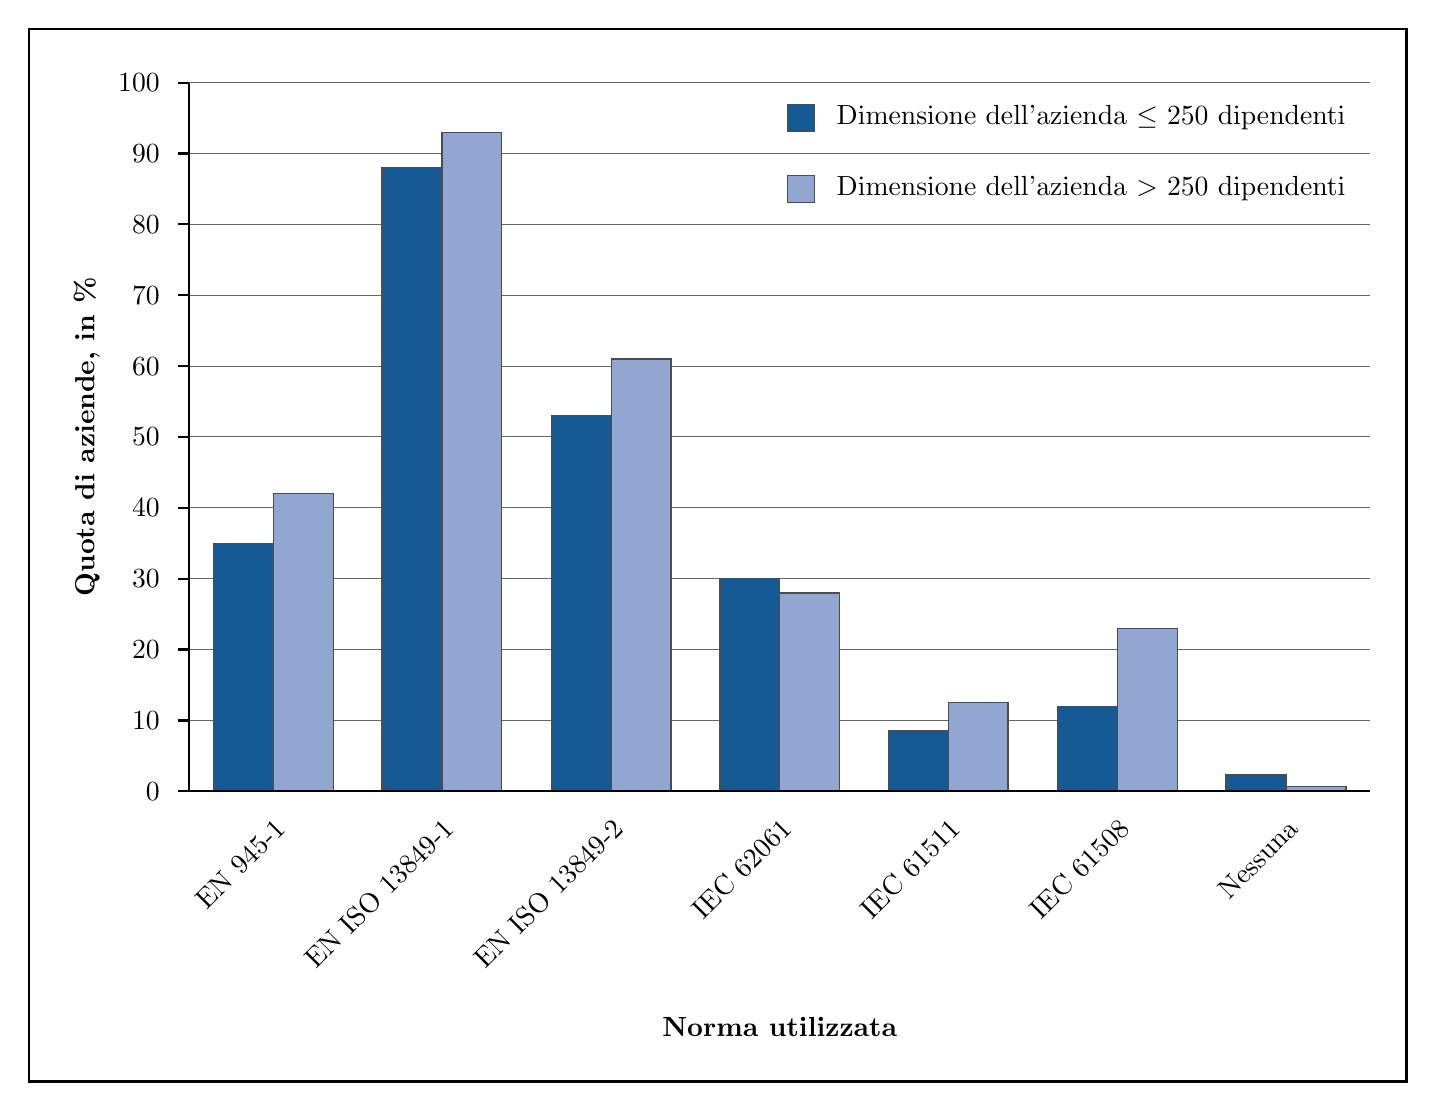
\begin{tikzpicture}[
  font=\normalsize,
  griglia/.style={draw=black!60, line width=0.4pt},
  asse/.style={draw=black, line width=0.8pt},
  barra/.style={draw=black!70, line width=0.5pt}
]

%--------------------------------------------------------------
% Griglia orizzontale e scala verticale (da 0 a 100%)
%--------------------------------------------------------------
\foreach \p in {0,10,...,100} {
  \draw[griglia] (0,{\p*0.09}) -- (15.0,{\p*0.09});
  \draw[asse] (-0.14,{\p*0.09}) -- (0,{\p*0.09});
  \node[anchor=east] at (-0.25,{\p*0.09}) {\p};
}

%--------------------------------------------------------------
% Barre: per ciascuna norma, aziende fino a 250 e oltre 250
%--------------------------------------------------------------
\foreach \cx/\va/\vb in {1.07/35/42, 3.21/88/93, 5.36/53/61,
                         7.50/30/28, 9.64/8.5/12.5, 11.79/12/23,
                         13.93/2.3/0.7} {
  \fill[blusc] ({\cx-0.76},0) rectangle (\cx,{\va*0.09});
  \draw[barra] ({\cx-0.76},0) rectangle (\cx,{\va*0.09});
  \fill[bluch] (\cx,0) rectangle ({\cx+0.76},{\vb*0.09});
  \draw[barra] (\cx,0) rectangle ({\cx+0.76},{\vb*0.09});
}

%--------------------------------------------------------------
% Assi e loro denominazioni
%--------------------------------------------------------------
\draw[asse] (0,0) -- (0,9.0);
\draw[asse] (0,0) -- (15.0,0);

\foreach \cx/\lab in {1.07/EN 945-1, 3.21/EN ISO 13849-1,
                      5.36/EN ISO 13849-2, 7.50/IEC 62061,
                      9.64/IEC 61511, 11.79/IEC 61508, 13.93/Nessuna}
  \node[rotate=45, anchor=north east] at (\cx,-0.15) {\lab};

\node[rotate=90] at (-1.30,4.5) {\bfseries Quota di aziende, in \%};
\node[anchor=north] at (7.50,-2.75) {\bfseries Norma utilizzata};

%--------------------------------------------------------------
% Legenda
%--------------------------------------------------------------
\fill[blusc] (7.60,8.38) rectangle (7.94,8.72);
\draw[barra] (7.60,8.38) rectangle (7.94,8.72);
\node[anchor=west] at (8.10,8.55)
  {Dimensione dell'azienda $\leq$ 250 dipendenti};

\fill[bluch] (7.60,7.48) rectangle (7.94,7.82);
\draw[barra] (7.60,7.48) rectangle (7.94,7.82);
\node[anchor=west] at (8.10,7.65)
  {Dimensione dell'azienda $>$ 250 dipendenti};

%--------------------------------------------------------------
% Cornice
%--------------------------------------------------------------
\draw[draw=black, line width=1pt]
  ([shift={(-0.45,0.45)}]current bounding box.north west) rectangle
  ([shift={(0.45,-0.45)}]current bounding box.south east);

\end{tikzpicture}
